% % Einordnung in SIL, MIL, HIL, was ist Testen allgemein?
% % Weiter in black box, dynamisch und funktional ( ist die Einordnung der Äquivalenzklassen)
% % Grob das ganze Umfeld erklären und Sachen wie black box testing näher erklären
% %in the Loop erklären
% Antriebsfunktionen elektrischer Maschinen sind als Software geschrieben, laufen auf einer 
% Hardware und übernehmen die Steuerung der Maschine. Das macht ein eingebettetes System aus.
 % % zu testen. Es 
% % Die Steuerung elektrischer Maschinen ist ein eingebettetes System, wobei der Motor von einem
% % Mikrocontroller gesteuert wird.
% Ein eingebettetes System ist in der Regel ein in-the-Loop System. In einem in-the-Loop System bilden Ausgänge des Systems
% eine Rückkopplung zu den Eingängen. Dies muss auch beim Testen berücksichtigt werden.

% Software-in-the-Loop bedeutet, dass die Software als in the Loop System getestet wird, wobei die Hardware
% simuliert wird. Bei Hardware-in-the-Loop hingegen ist die Hardware vorhanden und die Software wird, während
% es auf der Hardware ausgeführt wird, getestet.
% SIL ist in der Entwicklung bedeutend, da es keine Hardware zum Testen benötigt und schon in den 
% frühen Phasen der Entwicklung getestet werden kann\parencite[S.1 f.]{silest}. Je länger ein Fehler unentdeckt bleibt und nicht
% behoben wird, umso teurer wird dieser Fehler.

% Diese Arbeit handelt davon TPT als Programm einzusetzen, um einen Schnittstellentest zu überführen und ein
% neues Testkonzept mit Äquivalenzklassen zu erarbeiten.
% Diese Arbeit handelt von der Entwicklug eines Konzepts für Äquivalenzklassen und Überführung eines 
% Schnittstellentests. Beides in TPT.
In der Abteilung Softwareentwicklung elektrische Antriebsfunktion bei ZF, in der ich für die Bachelorarbeit tätig bin,
wird nach dem V-Modell entwickelt (siehe Abbildung 1.1).\par
\begin{figure}[h]
\centering
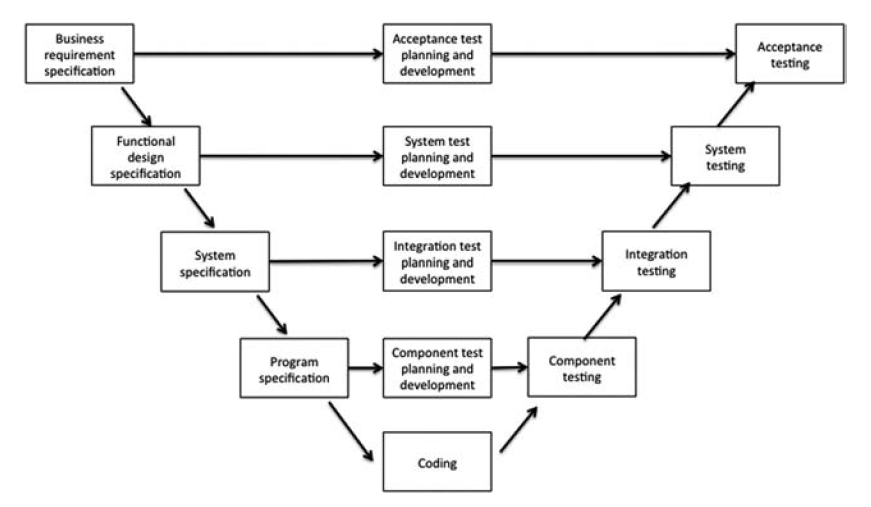
\includegraphics[scale=1.2,]{Bilder/VModell.png}
\caption{V-Modell \parencite[S. 68]{agiletesting}}\label{fig:VModell}
\end{figure}
Ein Merkmal des V-Modells ist, dass jede Stufe der Entwicklung einen dazugehörigen Test besitzt.
Die folgenden Testebenen beschreiben die einzelnen Teststufen \parencite[S. 41 f., S. 51]{integration}:
\begin{description}
\item[Komponententest] Es wird eine Komponente isoliert von der Software - funktional und strukturell - getestet. % \parencite[S. 41]{integration}
\item[Integrationstest] Es ist ein Test, der das Zusammenspiel bereits getesteter Komponenten überprüft. %  \parencite[S. 51]{integration}. 
\item[Systemtest] Es wird die Funktionsfähigkeit des ganzen Systems getestet. Dazu zählen auch Performanz-, Stress und Robustheitstests.
\item[Abnahmetest] Mit diesem Test wird überprüft, ob die Erwartungen der Anwender erfüllt werden. Der Test soll
unter realen Einsatzbedingungen stattfinden.
\end{description}
%Im Komponententest wird eine Komponente isoliert vom Rest der Software getestet. %\parencite[S.41]{integration}.
%Die Komponente wird funktional und strukturell getestet \parencite[S. 41]{integration}.
% Das ist der erste Test nach der Implementation.
% Der Komponententest zeichnet sich aus, dass einzelne elementare Programmbausteine isoliert getestet werden.
% Im Modultest bzw. Komponententest (unit test) werden einzelne elementare Programmbausteine
% isoliert getestet, oft vom jeweiligen Entwickler selbst. Die Bausteine bzw. Testobjekte
% können dabei auch zusammengesetzt sein. Der Tester hat in der Regel Zugang zum Quellcode,
% sodass in dieser Teststufe sehr entwicklungsnah gearbeitet wird und es sind somit
% sowohl Black-Box- als auch White-Box-Verfahren anwendbar.
%Der Integrationstest ist ein Test, der das Zusammenspiel bereits getesteter Komponenten überprüft \parencite[S. 51]{integration}. 
%Fehler in den Schnittstellen sollen hier aufgedeckt werden.
% Wichtig:
% Es gibt verschiedene Integrationsstufen, die der Reihe nach getestet werden.(hier Integrationsstufen aufzählen).
%Hier Erklärung Integrationstest und Erklärung Komponententest einfügen.
%Jede Stufe der Entwicklung besitzt einen dazugehörigen Test.
Der Schnittstellentest, in dem die Signalverbindungen zwischen Komponenten überprüft werden, ist ein Teil des 
Integrationstests \parencite[S. 51, S. 217]{integration}.
Der Äquivalenzklassentest ist als funktionaler Test im Komponententest wiederzufinden \parencite[S. 41 f.]{integration}\parencite[S. 114 ff.]{equiinformatic}.

Wie der Äquivalenzklassentest einzuordnen ist, wird in Abbildung 1.2 deutlich.
Dieses Diagramm ist nicht vollständig, sondern soll nur als Einordnung dienen.
Eine Art der Analyse in der Software ist eine dynamische Analyse, eine weitere ist die statische Analyse.
In der dynamischen Analyse
wird der Code ausgeführt, in der statischen hingegen nicht. Eine Art der dynamischen Analyse ist funktional, eine weitere Art ist strukturell.
In der funktionalen Analyse wird das System als Kasten betrachtet, sprich Informationen über den Programmcode sowie
der inneren Struktur sind nicht von Bedeutung. Deshalb wird es auch als Blackbox-Testverfahren bezeichnet.
In der strukturellen Analyse hingegen wird der innere Ablauf im Testobjekt analysiert. Der Blickwinkel wandert
in das System. Es wird auch Whitebox-Testverfahren genannt.
Ein funktionaler Test ist der Äquivalenzklassentest. 
Ein weiterer ist die Grenzwertanalyse \parencite[S. 114 ff.]{equiinformatic}\parencite[]{dynamischeanalyse1}\parencite[]{dynamischeanalyse2}.
Die Grenzwertanalyse eignet sich hervorragend, um sie mit anderen Tests wie dem Äquivalenzklassentest 
zu kombinieren \parencite[S. 36]{integration}.\par
\begin{figure}[h]
\centering
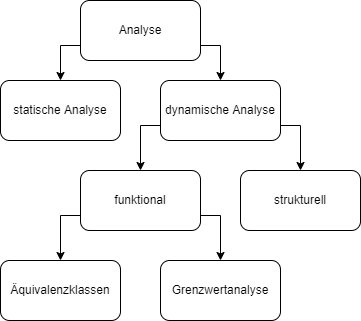
\includegraphics[scale=0.9,]{Bilder/Einordnung.drawio.png}
\caption{Einordnung der Äquivalenzklassen \parencite[]{dynamischeanalyse1}\parencite[]{dynamischeanalyse2}\parencite[S. 114 ff.]{equiinformatic}}
\end{figure}



% Schnittstellentest, Teil des Integrationstests.
% Äquivalenzklassentest ist Komponententest nach Abbildung V Modell.
% Analysearten Äquivalenzklassentest:
% dynamisch, statisch. Bla bla erklären nach Abbildung (Einordnung der Äquivalenzklassen)


% Verifikation und Validation umfasst 30-50% des Entwicklunsgaufwands
% Oftmals erst möglich, wenn Hardware vorhanden ist
% Keine Hardware: geringe Parallelisierbarkeit Entwicklung von Hard und Software
% Abhilfe: SIL
% Verifikation erschwert durch minimale Software-Schnittstellen
% Ausgänge von embedded systems Rückkopplung auf eigene Eingänge
% Software kann nicht losgelöst von technischem Umfeld getestet werden
% Untersuchung des Regelkreises notwendig(SIL ist Closed Loop, nicht open loop)
% Besonders wichtig: Test der Auswirkungen von Sensor und Aktuator Fehlverhalten
% SIL: Nachbildung des umgebenden technischen Systems als eine realistische und ausführbare Software-Simulation
% Vorteile: kostengünstiger, umfassender, wiederholbar, automatisierbar, rückverfolgbar






% SIL wird eingesetzt, da es viel 
% Besonders wichtig ist das Fehlverhalten von Sensoren und Aktuatoren zu testen.
% Test der Auswirkungen von Sensor und Aktuator Fehlverhalten


% \begin{figure}[h]
% \centering
% 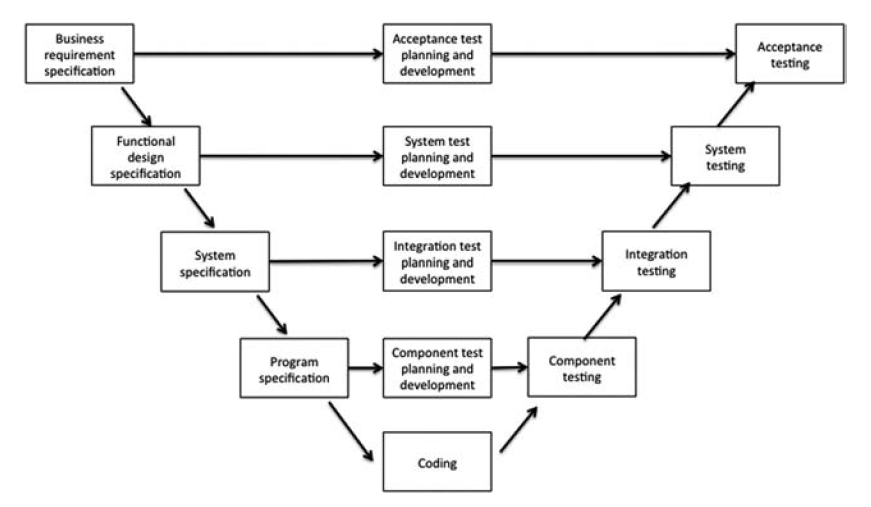
\includegraphics[scale=1.2,]{Bilder/VModell.png}
% \caption{V-Modell}
% \end{figure}
% \begin{figure}[h]
% \centering
% 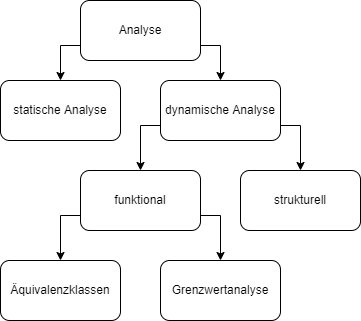
\includegraphics[scale=0.9,]{Bilder/Einordnung.drawio.png}
% \caption{Einordnung der Äquivalenzklassen}
% \end{figure}



% Quelle über dynamischer Test,black box (Äquivalenzklassen): Basiswissen\_Softwaretest...pdf\\

% % Von Y:\Bachelor\Bachelorarbeit\Basiswissen_Softwaretest_Aus-_und_Weiterbildung_zu..._----_(Pg_131--193).pdf

% % Bis Seite 148 geht es um Blackbox-Verfahren

% % Ziel des Testens: Nachweis der Erfüllung der festgelegten Anforderungen

% Dynamischer Test -> Blackbox -> Äquivalenzklassen\\

% Systematische Erstellung von Testfällen:
% % Blackbox Verfahren und whitebox Verfahren
% % "Die vorausgesagten Ergebnisse (Ausgaben, Änderung von internen
% % Zuständen usw.) müssen vor der Ausführung der Testfälle feststehen
% % und dokumentiert werden."
% % (In Softcar, der setpoint wird berechnet durch die Eingangswerte
% % Danach wird überprüft, ob das Programm auf das gleiche Ergebnis wie der setpoint gekommen ist)

% "Bei den Blackbox-Verfahren wird das Testobjekt als schwarzer
% Kasten angesehen. Über den Programmtext und den inneren Aufbau
% sind keine Informationen notwendig."\\

% "Bei den Whitebox-Verfahren wird auch auf den Programmtext
% zurückgegriffen. Während der Ausführung der Testfälle wird der
% innere Ablauf im Testobjekt analysiert (der Point of Observation liegt
% innerhalb des Testobjekts)."\\

% Blackbox: spezifikationsbasiertes Testentwurfsverfahren\\

% Whitebox: strukturelles Testverfahren\\

% dynamischer vs statischer Test\\

% Diagramm zeichnen mit der Einordnung von den unterschiedlichen Testarten(dynamisch, statisch, black box etc.)


% % Trends in Software Testing

% % SILreliability
% % SILreliability Vergleich von sil und hil, Trend geht dazu, dass mehr Hardware Sachen mit Software gelöst werden, V Modell zeigt sil ist für module und auch Integrationstest, Vorteil von sil gegenüber Hil ist, dass mit sil kein corrupted data entstehen kann (unter 4. Results)

% % \begin{lstlisting}
% % Virtual platforms von Software-in-the-Loop_simulation_of_embedded_control_applications_based_on_Virtual_Platforms.pdf
% % \end{lstlisting}
% % Ist ein Trend zur embedded software Entwicklung

% % "Another advantage
% % of using virtual platforms in the early stage of the software
% % development is that they allow observing the behavior of the
% % entire system which leads to excellent debugging options
% % compared to the “black box”-like behavior of embedded
% % devices."


% % Another advantage
% % of using virtual platforms in the early stage of the software
% % development is that they allow observing the behavior of the
% % entire system which leads to excellent debugging options
% % compared to the “black box”-like behavior of embedded
% % devices.